\documentclass[a4paper,14pt]{extarticle} %extrarticle
\usepackage[T2A]{fontenc}
\usepackage[utf8]{inputenc}
\usepackage[russian,english]{babel}
\usepackage[pdftex,unicode]{hyperref}
%\usepackage{pscyr}
\usepackage{cmap}
\ifx\pdfoutput\undefined
\usepackage{graphicx}
\else
\usepackage[pdftex]{graphicx}
\fi

\usepackage{amstext}
\usepackage{amssymb}
\usepackage{amsmath}
\usepackage{lscape}
\usepackage{makecell}
\usepackage{multirow}
\usepackage{multicol}
\usepackage{ulem}
\usepackage{indentfirst}
\setcounter{tocdepth}{3}
\usepackage{url} % для url'ов

% выставляем параметры страниц
\usepackage{geometry}
\geometry{verbose,a4paper,tmargin=2cm,bmargin=2cm,lmargin=2.5cm,rmargin=1cm}

% меняем шрифт на Times New Roman
%\usepackage{times}
%\renewcommand{\rmdefault}{ftm}
%\renewcommand\theadfont{\normalsize}

% меняем шрифты
%\renewcommand\large{\@setfontsize\large{15.5}{17}}
%\renewcommand\Large{\@setfontsize\Large{16.5}{19}}


\linespread{1.3} % 1,5
\graphicspath{{../images/}}

\begin{document} % начало документа
\sloppy

\begin{titlepage} % начало титульной страницы

\thispagestyle{empty}

\begin{center}
	\small{
    	\textbf {
        	Министерство образования и науки Российской Федерации \\
            Государственное образовательное учреждение высшего профессионального образования \\
            ДАЛЬНЕВОСТОЧНЫЙ ГОСУДАРСТВЕННЫЙ УНИВЕРСИТЕТ \\
            \smallskip \hrule height 2pt \smallskip \hrule \smallskip
            ИНСТИТУТ МАТЕМАТИКИ И КОМПЬЮТЕРНЫХ НАУК \\
            Кафедра информатики \\
        }
    }
    \vspace{1cm}
    Антонов Алексей Евгеньевич \\
    \vspace{1cm}
    РЕАЛИЗАЦИЯ АЛГОРИТМА РАСКРАСКИ ВОКСЕЛЕЙ С ИСПОЛЬЗОВАНИЕМ OpenCL \\
    \vspace{1cm}
    \textbf {ДИПЛОМНАЯ РАБОТА} \\
    по основной  образовательной программе подготовки специалистов\\
    по направлению 010501.65 – прикладная математика и информатика

	\vspace{4cm}

\end{center}
\small{
\begin{multicols}{2}
    \verb""\\
    \bigskip
    \verb""\\
    \bigskip
    \verb""\\
    \bigskip
    
    \noindent Защищена в ГАК с оценкой \\
    \rule{4cm}{0.5pt} \\
   Секретарь ГАК \\
   \rule{4cm}{0.5pt} \rule{4cm}{0.5pt} \\
   <<\rule{1cm}{0.5pt}>> июня 2010г.
        
    \noindentСтудент гр. 258  \rule{4cm}{0.5pt}  \\
    Руководитель ВКР заведующий лабораторией \\
    машинной графики ИАПУ ДВО РАН, д.т.н.\\
    \rule{4cm}{0.5pt} В.А.Бобков \\
    <<\rule{1cm}{0.5pt}>> \rule{4cm}{0.5pt} 2010г.

    \verb""\\
    \bigskip
    \verb""\\
    \bigskip
    \verb""\\
    \bigskip
    
\end{multicols}

\vfill

\begin{center}
    г. Владивосток\\
    2010
\end{center}
}
\end{titlepage} % конец титульной страницы

\setcounter{page}{2}
% меняем оформление оглавления
\begin{center}
\renewcommand{\contentsname}{Оглавление}
\tableofcontents % содержание
\end{center}

\newpage

\section{Введение}

\subsection{Глоссарий}
\textbf{Воксел} -- элемент объёмного изображения, содержащий значение элемента растра в трёхмерном пространстве. Вокселы являются аналогами пикселов для трехмёрного пространства.~\cite{wiki_voxel}

\textbf{Кроссплатформенное программное обеспечение} -- программное обеспечение, работающее более чем на одной аппаратной платформе и/или операционной системе.~\cite{wiki_crossplatfom}

\textbf{ПК} -- персональный компьютер.

\textbf{Реконструкция} -- построение объемной модели реального объекта.

\textbf{Фреймворк} -- в информационных системах структура программной системы; программное обеспечение, облегчающее разработку и объединение разных компонентов большого программного проекта. В его состав могут входить вспомогательные программы, библиотеки кода, язык сценариев и проч.~\cite{wiki_framework}

\subsection{Описание предметной области}
Потребность в реалистичном отображении окружающего мира увеличивает значимость трехмерного (3D) моделирования -- построения компьютерных моделей объектов. 3D модели облегчают планирование, контроль и принятие решений во многих отраслях. Например, если в ходе эксплуатации модели требуется внести коррективы, компьютерный объект позволит это сделать максимально быстро.

Особенно сложной проблемой является создание точных моделей объектов из реального мира.~\cite{komarova_voxel_coloring} Как быстро выяснилось, человеческий глаз очень легко определяет погрешности в синтезированных изображениях хорошо известных ему в повседневной жизни объектов.

Вот несколько примеров объектов, требующих реконструкции:
\begin{enumerate}
\item Здания и строения
\item Предприятия со сложной структурой (нефтегазоперерабатывающие комплексы, химические предприятия и т.д.)
\item Дороги и дорожные объекты (мосты, путепроводы, прилегающая зона)
\item Открытые и закрытые горные разработки
\item Рельефы местности
\end{enumerate}

\subsubsection{Методы построения моделей объектов}
На данный момент существует три основных способа получения модели объекта:
\begin{itemize}
\item Использование активных методов (например, лазерных сканеров, позволяющих с высокой точностью определить расстояние от лазера до поверхности объекта)
\item Вручную с помощью программ трехмерного моделирования (например, Blender, 3D Studio Max)
\item Автоматическая реконструкция объекта по набору изображений и другой известной о нем информации
\end{itemize}

Сканеры -- современное средство измерения, позволяющее производить исполнительную съемку сложных объектов, там, где проходит множество пересечений на различных уровнях. Причем вступать в контакт с самим объектом не требуется. Сканер формирует модель по десяткам тысяч точек, при этом положение каждой из них определяется с точностью от 2--3 мм до 2 см. Наземные сканеры используются для создания моделей зданий, заводов, кварталов и других больших сооружений. Дальность сканера составляет порядка 200 метров, на таком расстоянии он может определять объекты с точностью шага до 0.5 см. Современные сканеры в состоянии сканировать окружающую действительность с поворотом на 360 градусов, что позволяет сканировать сразу несколько зданий. Сшивка отдельных сканов выполняется посредством специальных марок или характерных точек рельефа. Такой метод обеспечивает высокое качество проектирования, приближая его к реальности. Недостатками использования сканера являются высокая стоимость оборудования (от 50 тыс. долл.~\cite{laser_scanner}), необходимость в высококвалифицированных специалистах, способных это оборудование обслуживать, а так же невозможность реконструкции динамических сцен.~\cite{komarova_voxel_coloring}

Второй подход требует больших затрат усилий и времени, что вытекает в высокую стоимость и длительные сроки разработки модели.

В третьем подходе в качестве исходных данных используют только фотографии или последовательности изображений объектов, полученные в естественном освещении, или приближенном к нему (в свете обычных ламп). Такой подход считается наиболее перспективными, так как позволяет строить модели динамических сцен, в которых могут участвовать люди.

\subsection{Неформальная постановка задачи}
Создание кроссплатформенного приложения, использующего для реконструкции объекта алгоритм раскраски вокселей по методу множества гипотез~\cite{multi_hypothesis} и способного задействовать все возможности современного ПК. Из поставленных условий вытекает еще одна задача -- распараллеливание существующего алгоритма.

\subsection{Математические методы}
В качестве базового, для построения модели объекта, используется алгоритм раскраски вокселей по методу множества гипотез~\cite{multi_hypothesis}.

\subsection{Обзор существующих методов решения}

На текущий момент была найдена только одна, находящаяся в открытом доступе, реализация алгоритма раскраски вокселей -- Voxel Coloring Framework~\cite{voxel_coloring_framework}. К её достоинствам можно отнести распространение под академической свободной лицензией~\cite{academic_free_license}. Однако данная реализация обладает следующими недостатками:
\begin{itemize}
\item Работает только в операционной системе семейства MS Windows
\item Для работы необходим пакет Matlab
\item Не использует вычислительные возможности современных графических адаптеров
\end{itemize}

\section{Методы построения моделей объектов}
На данный момент существует три основных способа получения модели объекта:
\begin{itemize}
\item Использование активных методов (например, лазерных сканеров, позволяющих с высокой точностью определить расстояние от лазера до поверхности объекта)
\item Вручную с помощью программ трехмерного моделирования (например, Blender, 3D Studio Max)
\item Автоматическая реконструкция объекта по набору изображений и другой известной о нем информации
\end{itemize}

Сканеры -- современное средство измерения, позволяющее производить исполнительную съемку сложных объектов, там, где проходит множество пересечений на различных уровнях. Причем вступать в контакт с самим объектом не требуется. Сканер формирует модель по десяткам тысяч точек, при этом положение каждой из них определяется с точностью от 2--3 мм до 2 см. Наземные сканеры используются для создания моделей зданий, заводов, кварталов и других больших сооружений. Дальность сканера составляет порядка 200 метров, на таком расстоянии он может определять объекты с точностью шага до 0.5 см. Современные сканеры в состоянии сканировать окружающую действительность с поворотом на 360 градусов, что позволяет сканировать сразу несколько зданий. Сшивка отдельных сканов выполняется посредством специальных марок или характерных точек рельефа. Такой метод обеспечивает высокое качество проектирования, приближая его к реальности. Недостатками использования сканера являются высокая стоимость оборудования (от 50 тыс. долл.~\cite{laser_scanner}), необходимость в высококвалифицированных специалистах, способных это оборудование обслуживать, а так же невозможность реконструкции динамических сцен.~\cite{komarova_voxel_coloring}

Второй подход требует больших затрат усилий и времени, что вытекает в высокую стоимость и длительные сроки разработки модели.

В третьем подходе в качестве исходных данных используют только фотографии или последовательности изображений объектов, полученные в естественном освещении, или приближенном к нему (в свете обычных ламп). Такой подход считается наиболее перспективными, так как позволяет строить модели динамических сцен, в которых могут участвовать люди.

Существует целый набор подходов, на основе которых разрабатываются методы реконструкции по последовательности изображений. Среди них реконструкция моделей по набору силуэтов объекта и раскраска вокселей на основе правила согласования цветов.

\subsection{Силуэтные методы}
\subsubsection{Видимая оболочка}
Сопоставим каждому исходному изображению битовую карту. Если пиксель изображения соответствует объекту, то бит ставится в 1, в противном случае в 0. Тогда силуэтом объекта на данном изображении называется множество всех равных 1 битов. Силуэтные методы восстанавливают геометрическую модель объекта только по его силуэтам. Эти методы также часто называются методами пересечения объемов (volume intersection). В 1991 году Лаурентини в свое работе доказал, что данные методы позволяют получить только <<видимую оболочку>> (visual hull) объекта. Видимой оболочкой называют наибольший объект, чей силуэт с любой точки обзора совпадает с силуэтом исходного объекта из этой же точки. Силуэтные методы в качестве исходных данных используют конечный набор изображений, поэтому они реконструируют <<предполагаемую видимую оболочку>>. Ее можно представить как пересечение телесных конусов, с вершиной в точке расположения камеры, и сечениями - силуэтами. Такие конусы называются силуэтными конусами.
\renewcommand{\figurename}{Рис.}
\begin{figure}[h]
\center
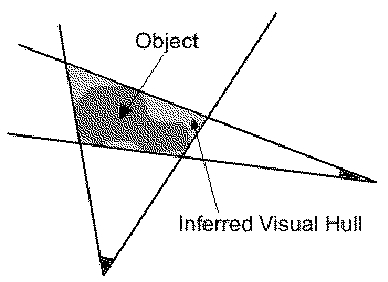
\includegraphics[scale=0.5]{vh}
\caption{Предполагаемая видимая оболочка}
\end{figure}

Предполагаемая видимая оболочка обладает следующими свойствами:
\begin{itemize}
    \item Каждый объект целиком содержится внутри любой своей предполагаемой видимой оболочкой
    \item Размер (объем) предполагаемой видимой оболочки уменьшается с увеличением количества исходных изображений
\end{itemize}

\subsubsection{Силуэтные методы для вокселного представления}
Первый силуэтный метод был разработан Мартином и Аггагвалом в 1983~\cite{aggarwal}. С помощью обычного порогового фильтра яркости (intensity) они отделяли изображения фона от объекта. Морфологическая обработка полученного бинарного изображения позволяла определить силуэт. В качестве представления модели они выбрали модификацию вокселного - колонное представление. вокселный куб задавался набором столбиков вокселей, перпендикулярный одной заданной плоскости. Каждый столбик (колонна) в этом случае описывается глубиной первого и последнего воксела в столбике. Отрезки, соответствующие столбикам, проецировались на исходные силуэты, определялись точки пересечения проекций с силуэтом, а затем столбики обрезались - удалялась часть, проецирующаяся вне силуэта.
\begin{figure}[h]
\center
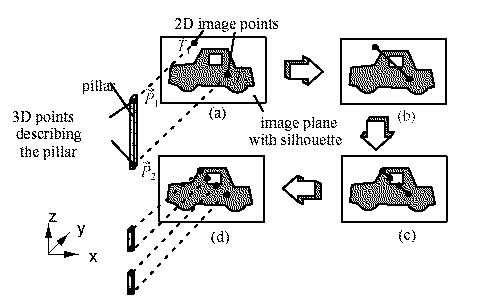
\includegraphics[scale=0.5]{pillar}
\caption{Удаление части вокселного столбца, проецирующегося вне силуэта объекта}
\end{figure}

В 1984-1986 годах Чин исследовал объемные представления на основе окто-деревьев~\cite{chien}. Исходными данными для его метода были три бинарных изображения полученные с ортогональных направлений визирования. Они затем преобразовывались в квадродеревья, и объединялись в одно окто-дерево. Такие строгие ограничения (ортогональность) на исходные изображения были главным недостатком это метода. В 1984 году Шнайер также предложил строить окто-деревья из сегментированных изображений, но реализация его идей так и не был осуществлена.

В 1987 году Потмесил разработал усовершенствованный алгоритм для реконструкции объектов по набору изображений с произвольно расположенных перспективных камер. Его алгоритм состоит из трех основных стадий. На первой стадии для каждого силуэта строится объемный конус в представлении окто-деревом. На второй эти конусы объединяются в модель. На третьей стадии вначале определяются границы каждого объекта, по соседним точкам рассчитываются нормали в каждой точки поверхности объектов. Затем каждой точке назначается определенный цвет из исходных изображений. Если данная точка видна на нескольких изображениях, то ее цвет определяется путем усреднения~\cite{potmesil}. Аналогичный метод был предложен в 1990 году, но все тесты его метода были проведены на синтезированных изображениях.

Метод Сзилиски, опубликованный в 1993 году, также использует окто-деревья в качестве объемного представления~\cite{szeliski}. Хотя его подход кажется очень похожим на подход Потмесила, их отличия весьма существенны. Потмесил строит отдельное окто-дерево по каждому изображению, а Сзилиски использует одно окто-дерево, уточняемое постепенно по новым изображениям, что значительно повышает скорость работы алгоритма.

Во второй половине 90-х годов методы получение видимых оболочек были применены для построения динамических сцен по видеопотокам, получаемым с набора видеокамер. Моэцца описывает систему из 17 камер, наблюдающих за сценой размером 1*1*2 метра. Каждый кадр обрабатывался для получения бинарного изображения - отделения фона и переднего плана. Методы пересечения силуэтных конусов применялись для построения видимых оболочек в вокселном представлении по сохраненным видеопотокам (в реальном времени на это не хватало времени). Объем одного воксела составлял около 1 см. Из вокселной модели по методу изолиний строилась полигональная модель, для которой затем рассчитывалась текстура. Цвет текстуры получался взвешенным усреднением значений соответствующих пикселей в изображениях. В 1997 году эта технология была улучшена с помощью новых методов раскраски поверхностей.

Достоинством всех силуэтных методов является их мощность, ведь исходной информацией для них выступают калиброванные силуэты. Поверхность объекта, который запечатлен на изображениях, может не быть диффузной, а обладать, например, зеркальными свойствами.

Недостатков же у упомянутых выше методов несколько. Главным недостатком является невозможность точного представления формы объекта, может строиться только видимая оболочка объекта, форма которой во многих случаях отличается от формы объекта. Во вторых, при использовании отдельного вокселного представления возникают трудности с определением проекции вокселей на силуэты во время работы метода. Размеры вокселей могут быть значительны, и они будут пересекаться с границей силуэтов. В этом случае при любом выборе - прозрачным или непрозрачным объявляется обрабатываемый воксел - форма объекта представляется с погрешностью. Третий недостаток заключается в том, что эти силуэтные алгоритмы предназначены только для определения геометрической формы объекта, а не его текстуры. Цвет поверхности объекта необходимо рассчитывать отдельными методами. 

\subsubsection{Видимая оболочка на основе изображений}
В 2000 году была предложена идея видимой оболочки на основе изображений (image-based visual hull). Это разновидность многослойного изображения с глубиной. Для каждого пикселя изображения с силуэтом объекта хранится список заполненных отрезков. Если пиксель не входит в силуэт (т.е. принадлежит фону) это список пуст. В противном случае, список содержит интервалы пространства, принадлежащие видимой оболочке объекта. Каждый интервал представляет собой часть телесного конуса с вершиной в точке камеры и сечением-пикселем, т.е. часть видимой оболочки, проецирующейся в данный пиксель. Объединение всех таких интервалов дает нам дискретизацию видимого тела для данной точки обзора. Каждый интервал храниться в виде пары точек (ближняя и дальняя границы), заданных глубиной и цветом. Считается, что цвет любой точки интервала интерполируется по цветам граничных точек.
\begin{figure}[h]
\center
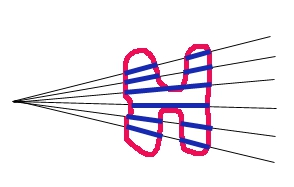
\includegraphics[scale=0.5]{ibvh}
\caption{Набор отрезков, составляющих видимую оболочку на основе изображений}
\end{figure}

Видимая оболочка на изображениях строится в исключительно в пространстве изображений, без создания каких-то объемных структур. Для каждого пикселя силуэта данного изображения строится луч, проходящий через точку камеры и центр пикселя. Этот луч затем проецируется на все остальные изображения. В каждом из них рассчитываются точки пересечения проекции и силуэта. Зная калибровку каждой из камер по точкам пересечения проекции и силуэта можно определить трехмерные координаты точек пересечения самого луча и видимой оболочки, отсортировать их по глубине и выделить интервалы, принадлежащие видимой оболочке. Для ускорения алгоритма может используется буфер проекций, хранящий уже спроецированные лучи и точки пересечения для них. Прирост в скорости получается за счет разницы в количестве возможных проекций и количестве обрабатываемых лучей.

\subsection{Согласование по цветам}
\subsubsection{Условие согласования по цветам}
Группа методов <<раскраски вокселей>> основана на условии согласовании по цветам (color consistency), впервые описанном Сайтцем в 1997 году. Используя это правило, можно определить, лежит ли данная точка на поверхности объекта, или нет. Предположим, что все поверхности наблюдаемых объектов - диффузны. Пусть камеры A и B наблюдают одну и ту же точку в пространстве С. Обозначим за P(C,A) и P(C,B) пиксели на полученных с камер А и B изображениях, соответствующих точке С. Если С - лежит на поверхности некоторого объекта, то цвета пикселей P(C,A) и P(C,B) приблизительно равны, тогда С называется согласованной по цвету. Если же точка С - воображаемая точка в пустом пространстве, то цвета обоих пикселей соответствует цветам двух различных точек D и Е, а значит, скорее всего будут различны. 
\begin{figure}[h]
\center
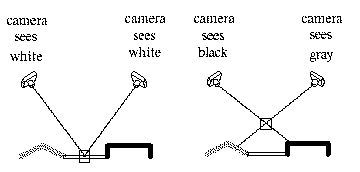
\includegraphics[scale=0.7]{consistency}
\caption{Случаи выполнения и невыполнения условия согласования по цветам}
\end{figure}

На данный момент, все методы восстановления моделей с использованием согласования по цветам используют вокселное представление и обладают одним общим недостатком. Связан он с обработкой резких цветовых переходов на поверхностях объекта, которые часто встречаются в реальном мире. Воксели, соответствующие таким цветовым границам, будут скорее всего проецироваться в несогласованные по цветам пиксели. Для таких вокселей, тест на согласованность цветов может выдать отрицательный результат. Эта проблема может быть решена с помощью адаптивного изменения порогового значения, увеличивающегося, если воксел признается несогласованным только по пикселям отдельных изображений.

Однако, в некоторых случаях, когда резкий цветовой переход совпадает с углом объекта, проблема усугубляется. Хорошим примером этой проблемы является моделирование обычного кубика с разноцветными гранями. На изображениях одного и того же угла с разных сторон он будет виден под совершенно разными цветами. В этом случае, поднятие порога уже не спасает положение. воксел, соответствующий углу, признается несогласованным и отбрасывается. После этого, уже соседние с ним воксели могут быть помечены как несогласованные и удалены из модели. Таким образом, строится некорректная модель объекта. Эта проблема не упоминается в работах по моделированию по условию согласования цветов.
\begin{figure}[h]
\center
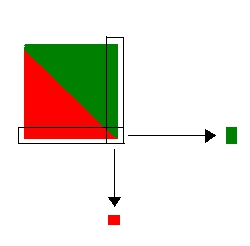
\includegraphics{cons_trouble}
\caption{Возможная ошибка согласования цветов}
\end{figure}

\subsubsection{Методы согласования по цветам с ограничением на расположение камер}
Первый метод, использующий согласование был разработан Фромхерцем в 1995 году. Он использовал идею согласованности по яркости в дополнение к основному алгоритму пересечения объемов. В 1997 году Сайтц и Дир продемонстрировали, что хорошо раскрашенные сцены могут быть восстановлены и с помощью одного метода согласования цветов, без использования пересечения объемов. Они назвали свой алгоритм - <<раскраска вокселей>> (voxel coloring).

По их методу берется вокселный куб, заключающий в себе всю восстанавливаемую сцену, и все воксели помечаются как непрозрачные. Затем последовательно проверяется каждый воксел на согласованность цветов. Если воксел не проходит этот тест, то он помечается как прозрачный (вырезается). Алгоритм завершается, когда все непрозрачные воксели признаются согласованными по цветам. Последним этапом является назначение каждому непрозрачному (не вырезанному) вокселю соответствующего цвета. Визуализированное изображение полученной вокселной сцены будет достаточно точно совпадать с исходными изображениями.

На промежуточных стадиях работы этого алгоритма еще не просмотренные непрозрачные воксели могут закрывать друг друга. Поэтому, чтобы проверить воксел на согласование цветов необходимо вначале определить его видимость (т.е. определить те изображения из исходных, на которых он виден в данный момент). Эта процедура применяется к каждому обрабатываемому вокселю, поэтому она должна быть максимально оптимизирована. Расчет видимости оказывается одной из самых хитрых задач при разработке алгоритмов на основе согласования по цвету, и для ее решения предлагались различные подходы.

Сайтц и Дир накладывали определенное ограничение на расположение камер, с которых получали исходных изображений, названное ими ограничением на порядок видимости (ordinal visibility constraint). Оно требовало такого расположения камер, чтобы все воксели могли быть просмотрены за один проход, в порядке от ближайших к самым удаленным относительно каждой камеры. Обычно такому требованию удовлетворяло расположения всех камер по одну сторону от сцены, и обход вокселного тело последовательно по слоям, от ближнего к дальнему. Поэтому воксели, которые могли загораживать другие, проверялись на согласованность в первую очередь. Это гарантировало то, что видимость каждого воксела не изменялась после его просмотра. Для каждого исходного изображения дополнительно задавалась битовая карта видимости (occlusion bit map). Вначале, все ее биты устанавливались равными нулю. Если проецирующийся в данный пиксель воксел помечался как согласованный и непрозрачный, то бит видимости для него устанавливался в 1.

Время восстановления сцены по алгоритму Сайтца и Дира пропорционально количеству вокселей в представлении сцены. Прок в 1998 году показал, что модификация их алгоритма с переменной разрешающей способностью (multiresolution) позволяет достичь в некоторых случаях десятикратного прироста в скорости. Вначале сцена восстанавливалась с низким разрешением. Некоторые воксели в этом случае помечались как пустые, т. к. лишь малую часть их объема занимали объекты сцены. Но если разбить такой большой воксел на несколько маленьких, то некоторые из маленьких окажутся почти полностью заполненными. Поэтому все соседние с невырезанными вокселами обратно добавляются в модель, и помечаются как непрозрачные. Такая модифицированная модель в низком разрешении направляется на последующую обработку. Каждый непрозрачный воксел разбивается обычно на 8 маленьких. Затем они все снова проверяются на согласованность цветов. Полученная промежуточная модель будет исходной точкой для следующей итерации алгоритма. Программа продолжает работать до тех пор, пока не будет получена модель в требуемом разрешении. Такой подход является развитием силуэтного метода и использует согласование цветов.

\subsubsection{Алгоритмы согласования по цветам с произвольным расположением камер}
граничение на порядок видимости, необходимое для корректной работы алгоритма закраски Сайтца и Дира, не позволяет камерам находится вокруг сцены. Поэтому некоторая часть сцены всегда остается невидимой, а значит и не может быть восстановлена. Это самый главный недостаток этого метода. Если же расположить камеры произвольно вокруг сцены, то не будет существовать такого порядка обхода вокселей, который бы гарантировал неизменность видимости после просмотра воксела. Поэтому необходимо просматривать все воксели несколько раз, пока видимость каждого воксела перестанет изменяться.

Если хоть один воксел во время текущего просмотра удаляется из модели, то видимость остальных вокселей считается изменившийся, и модель должна быть просмотрена еще раз.

Данный алгоритм будет работать корректно, если ни один воксел, который должен быть признан согласованным в результирующей модели не будет вырезан на предыдущих стадиях. В 1998 году Кутулакос сформулировал условие монотонности меры согласованности, при выполнении которого обеспечивается корректность его работы. Монотонность обозначает, что если множество вокселей было признано несогласованным, то любое их надмножество тоже будет несогласованным. Так как алгоритм может только удалять воксели, но не добавлять их в сцену, то видимость воксела может только повыситься, т.е. пиксели, из которых виден данный воксел в данный момент обязательно будут только подмножеством тех пикселей, из которых он будет виден в последующем. Так как алгоритм не удаляют те воксели, которые окажутся согласованными по цвету в результирующей модели, то говорится, что процесс удаления (<<вырезания>>) консервативен. Кроме того, Кутулакос и Сайтц доказали, что найденная модель будет содержать в себе любую модель данной сцены из согласованных вокселей. Такая модель называется фото-оболочкой.

Кутулакос и Сайтц описали реализацию подобного алгоритма, получившего название <<Резьба по пространству>> (space carving). Для определения согласованности вокселей используется обычный алгоритм раскраски вокселей, в каждый момент времени просматривается один слой вокселей. Метод обеспечивает просмотр слоев от ближнего-к-дальнему относительно камер, используя в данный момент времени только изображения, полученных с камер расположенных по одну сторону от просматриваемой плоскости слоя. Поэтому, когда воксел просматривается, те из вокселей, которые могли его загораживать для используемых камер, уже были просмотрены. Так как процесс консервативен, то множество невырезанных вокселей в данный момент времени будет надмножеством вокселей искомого множества согласованных вокселей.

Однако восстановленная по методу Резьбы по пространству модель может содержать некоторые несогласованные по цвету воксели. Это происходит вследствие того, что при просмотре вокселей не рассматриваются изображения с камер, расположенных по другую сторону от плоскости слоя, даже если обрабатываемый воксел с них виден.

Существует также вариант этого метода для плохо калиброванных исходных изображений, который получил название Приближенная резьба по пространству (approximate). При оценке согласованности воксела по цвету, метод исследует цвет не отдельных пикселей, а круга из пикселей радиуса r в центре с точкой проекции воксела. Если цвета таких кругов совпадают в изображениях, то воксел признается r-согласованным и остается, в противном случае он вырезается. Параметр r выбирается с учетом качества калибровки изображений, чем выше точность калибровки, тем меньше может браться r. Соответственно, тем более точное приближение фото-оболочки может быть получено.

\subsubsection{Обобщенная раскраска вокселей}
В 1999 году был описан эффективный алгоритм расскраски вокселей, получивший название Обобщенной раскраски вокселей, в котором точно и полно рассчитывается видимость вокселей с учетом всех камер. Как также было показано, вычисление полной видимости позволяет получать более качественные модели по сравнению с обычным метом Резьбы по Пространству.

Всего было предложена два варианта этого алгоритма - первый использовал буферы элементов, а второй - многослойные буферы, разновидность многослойных изображений с глубиной. Эти структуры использовались для расчета видимости вокселей. Для каждого исходного изображения строится одна из описанных структур. В буфере элементов для каждого пикселя изображения указывается видимым в данном пикселе воксел модели. В многослойном изображении с глубиной записан отсортированный по глубине всех вокселей, которые проектируются в данный пиксель. Таким образом в многослойном изображении хранится больше информации чем в буфере элементов, что требует значительно больше памяти. Буфер элементов и многослойное изображение могуть быть получены с помощью визуализации по методу стандартного z-буфера. Это может быть сделано как программно, так и с помощью существующего аппаратного обеспечения. Видимость пикселей определяется следующим образом - просматриваемый воксел проецируется на все изображения, и если соответствующие проекциям метки в буфере элементов или многослойном изображении совпадают с идентификатором воксела, то он считается видимым.
\begin{figure}[h]
\center
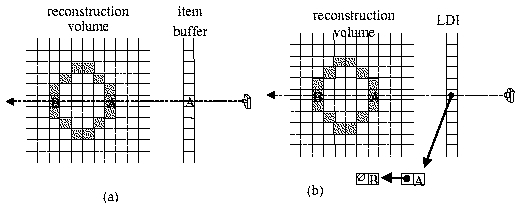
\includegraphics[scale=0.5]{generalized}
\caption{Обычный и многослойный буфер элементов}
\end{figure}

\subsubsection{Метод множества гипотез}
В работе Айсерта в 1999 году был предложен метод раскраски вокселей с множеством гипотез. Гипотеза - это возможная раскраска воксела. Таким образом, его алгоритм состоит из двух этапов. Первым идет этап назначения вокселам гипотез. На втором происходит удаление несогласованных вокселей и отбраковка ложных гипотез. Те из вокселей, которые признаются согласованными и составляют результирующую модель.

На первом этапе каждый центр воксела проецируется на все исходные изображения, и определяются цвета соответствующих пикселей. Полученные цвета сравниваются для каждой возможной пары изображений. Если по крайней мере на двух изображениях цвета согласуются, то он объявляется гипотезой. Новая гипотеза назначается вокселю. Согласованность цветов определяется путем расчета расстояния между цветами в пространстве RGB. Этот процесс повторяется для каждого воксела. На этом этапе никакой восстановленной модели еще нет, есть только начальный вокселный параллелепипед. Соответственно нет и никакой информации о видимости каждого воксела, а значит множество гипотез будут ложными, не соответствующим цветам поверхностей объекта.
\begin{figure}[h]
\center
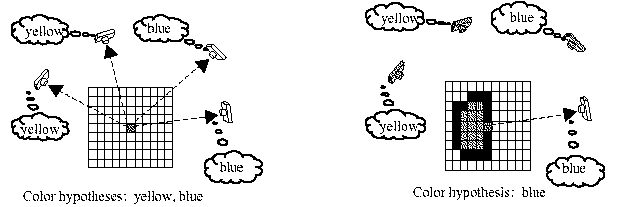
\includegraphics[scale=0.5]{multihyp}
\caption{Проверка выдвинутых гипотез о вокселе}
\end{figure}

Расчет видимости на втором этапе позволяет отбраковать ложные гипотезы. Для данной точки обзора обход вокселей осуществляется в порядке, совместимом с расчетом видимости. Каждый видимый воксел проецируется на изображения, и цвет пикселей, в которые проецируется центр воксела (или набора пикселей - проекции всего воксела) сравнивается с гипотезами, соответствующими данному вокселю. Если они не согласуются, то гипотеза признается ложной и отбраковывается. Если ложными признаются все гипотезы для данного воксела, воксел удаляется. Такое удаление воксела изменяет видимость остальных вокселей. Алгоритм продолжает работу пока для полученной промежуточной модели существуют гипотезы, которые можно признать ложными. Получившаяся после завершения работы модель является фото-оболочкой исходного объекта.

Этот метод очень похож на другие алгоритмы раскраски вокселей, Резьбы по пространству и Обобщенной раскраски вокселей. Главное их различие заключается в то, что в последних методах решение об удалении воксела из модели принимается на основе информации из всех исходных изображений вместе. В данном же методе, в текущий момент времени для отбраковки гипотез используется только одно из изображений. Это значительно упрощает расчет видимости, так как обход модели может проходить в порядке от ближнего-к-дальнему для одной камеры. Поэтому могут использоваться очень простые и не требующие много памяти битовые карты видимости. Недостатком же является необходимость в лишних вычислениях для расчета исходных гипотез для всех вокселей, включая и внутренние, даже те, которые в результирующей модели никогда не будут видны. В других методах, таких как в обобщенной раскраске, эти воксели никогда не будут обрабатываться. Кроме того, так как для каждого воксела обычно находится сразу несколько гипотез, алгоритму требуется в несколько раз больше памяти, чем другим методам на основе согласования по цветам.

\subsection{Выбор метода реконструкции}
Для данной работы был выбран метод множества гипотез. Представление объекта в данном подходе полностью объемное и не требуется никакого точного описания поверхности.  Подход основан на обработке проекций вокселной модели на множество изображений.  Изображения во всех камер одновременно участвуют в алгоритме.

В трехмерной реконструкции по изображениям с множества камер можно выделить два основных класса алгоритмов. Первый – вычисление карт глубины для двух и более изображений и преобразование этих карт в трехмерную модель. Восстановление карт глубины часто основано на соответствии точек изображения приближенной трехмерное модели либо на дополнительной информации от пространственных сенсоров. Второй класс алгоритмов основан на пересечении объемов и ссылается на информацию о силуэте объекта. Форма объекта представляется как пересечение телесных конусов, с вершинами в точках расположения камер, и сечениями-силуэтами. Такие конусы называются силуэтными конусами. 

Такие алгоритмы требуют точной сегментации объекта на изображении, что ограничивает набор кадров, так как объект должен легко отделяться от фона.

Метод множества гипотез совмещает преимущества обоих классов алгоритмов. При этом если фон сзади объекта однородный, то объект легко сегментируется. Если же фон неоднородный, метод также показывает хороший результат, так как использует цветовая информация.

К тому же, некоторые этапы метода не требуют строго последовательного обхода всех вокселей, что позволяет применить параллельные вычисления при его реализации.

\section{Неформальная постановка задачи}
В рамках данной работы были поставлены следующий задачи:
\begin{itemize}
\item Создание программной библиотеки, реализующей метод раскраски вокселей для реконструкции объектов, способной задействовать максимум из возможностей современного ПК.
\item Реализация набора приложений, показывающих возможности библиотеки.
\end{itemize}

Результаты работы предполагается предоставить в открытом доступе под <<Упрощенной BSD>> лицензией~\cite{bsd}.

\section{Обзор существующих методов решения}
Была найдена только одна, находящаяся в открытом доступе, реализация алгоритма раскраски вокселей -- Voxel Coloring Framework~\cite{voxel_coloring_framework}. К её достоинствам можно отнести распространение под академической свободной лицензией~\cite{academic_free_license}.
Эта реализация обладает следующими недостатками:
\begin{itemize}
\item Работает только в операционной системе семейства MS Windows
\item Для работы необходим пакет Matlab
\item Не использует вычислительные возможности современных графических адаптеров
\end{itemize}

\section{Требования к окружению}

\subsection{Требования к аппаратному обеспечению}
Необходимо наличие в системе устройств с поддержкой стандарта OpenCL~\cite{opencl_standart}. Список поддерживаемых устройств можно найти 
\begin{itemize}
\item для NVIDIA в \cite{opencl_nvidia_support}
\item для ATI в \cite{opencl_ati_support}
\item для S3 в \cite{opencl_s3_support}
\item для IBM в \cite{opencl_ibm_support}
\end{itemize}

\subsection{Требования к программному обеспечению}
Для работы приложения необходимо наличие в системе установленной библиотека Qt версии не ниже 4.6, а так же драйверов для устройств с поддержкой стандарта OpenCL версии 1.0.

\section{Спецификация данных}
\subsection{Формат метафайла}
Метафайл -- файл, используемый для сохранения и последующего восстановления информации о загруженных пользователем изображениях, введенных матрицах внешней и внутренней калибровки, объемлющем основной объект прямоугольнике. Этот файл записан в текстовом формате. Файл имеет следующую структуру:
\begin{itemize}
\item В первой строке находится беззнаковое целое число, обозначающее количество изображений, информация о которых записана в файле.
\item Далее идет три строки, содержащие по три элемента, разделенных пробелами. Каждый элемент -- число с плавающей точкой. Вместе они описывают матрицу внутренней калибровки камеры.
\item Далее идет информация об изображениях:
	\begin{itemize}
		\item имя файла с изображением, записанное в формате, совместимом с типом QString (см.~\cite{qt_qstring})
		\item прямоугольник, объемлющий основной объект, записанный в формате, совместимом с типом QRectF (см.~\cite{qt_qrectf})
		\item матрица внешней калибровки камеры для данного изображения, записанная в три строки по три числа с плавающей точкой в каждой.
	\end{itemize}
Количество таких блоков должно быть равным числу, записанном в первой строке файла.
\end{itemize}


\section{Функциональные требования}
Система должна позволять пользователю:
\begin{itemize}
\item загружать изображения
\item выделять основной объект
\item вводить матрицу внешней калибровки камеры для каждого изображения
\item вводить матрицу внутренней калибровки камеры
\item запускать выполнение алгоритма построения вокселной модели, на основе загруженных изображений
\item просматривать полученную воксельную модель объекта
\item сохранять и загружать метафайл
\item сохранять построенную воксельную модель
\item загружать для просмотра воксельную модель
\end{itemize}


\section{Требования к интерфейсу}
Система должна иметь приложение с графическим интерфейсом пользователя. Графический интерфейс должен предоставлять всю функциональность библиотеки.

\section{Проект}
\subsection{Средства реализации}
Для реализации приложения был выбран язык программирования C++, т.к. он очень распространен, что упрощает последующую поддержку приложения. К тому же, программы, написанные на этом языке, могут быть скомпилированы для очень большого количества платформ.

Для упрощения переноса приложения на другие платформы, был использован кроссплатформенный инструментарий разработки ПО под названием Qt. Он так же включает в себя инструментарий, необходимый для разработки кроссплатформенных приложений с графическим интерфейсом пользователя. Выбор этого инструментария позволяет уменьшить усилия, требуемые для реализации новой и поддержки имеющейся функциональности.

Для того, чтобы приложение могло задействовать как можно больше доступных ресурсов современных ПК, было решено использовать фреймворк OpenCL. Это позволит приложению задействовать ресурсы всех процессоров в многопроцессорных системах, а так же ресурсы современных видеокарт.
Для взаимодействия с OpenCL используется экспериментальный биндинг для языка C++~\cite{opencl_bindings}, который предоставляет ООП-интерфейс для доступа к OpenCL.

\section{Модули и алгоритмы}
Составляющими элементами системы являются библиотека covc и набор приложений:
\begin{itemize}
\item oclc
\item qcovc
\item ocl\_volume\_render
\end{itemize}


\subsection{Библиотека covc}
Библиотека covc содержит реализацию алгоритма раскраски вокселей методом множества гипотез.

\subsubsection{Программный интерфейс библиотеки}
Программный интерфейс библиотеки состоит из следующих функций:
\begin{itemize}
\item \textit{add\_image} -- добавление нового изображения
\item \textit{build\_voxel\_model} -- запуск алгоритма
\item \textit{get\_voxel\_model} -- получение результирующей вокселной модели
\item \textit{prepare} -- инициализация библиотеки
\item \textit{set\_camera\_calibration\_matrix} -- ввод матрицы внутренней калибровки камеры
\item \textit{set\_number\_of\_images} -- ввод количества изображений
\item \textit{set\_resulting\_voxel\_cube\_dimensions} -- ввод размерностей результирующей вокселной модели
\end{itemize}

\subsection{Алгоритм раскраски вокселей}
Все операции в процессе реконструкции производятся над вокселами, которые уникальны для трехмерной модели объекта, а не над пикселями, которых несколько для одного воксела. Поэтому не нужно специально вычислять точки соответствия и по ним вычислять карту глубины.

В реализованном алгоритме четыре этапа:
\begin{enumerate}
\item Вычисление объемлющего трехмерного куба объекта
\item Инициализация вокселей, назначение каждому вокселю гипотез
\item Первоначальная отбраковка ложных гипотез
\item Дальнейшая проверка гипотез на соответствие по всем изображениям и  удаление ложных гипотез
\end{enumerate}

\subsubsection{Вычисление объемлющего трехмерного куба объекта}
В начале работы программы можно ограничить пространство, в котором располагается реконструируемый объект. Для этого пользователь на изображениях выделяет рамкой объект. Затем, используя калибровочные данные, вычисляется объемлющий объект объем (bounding volume). Для его расчета на каждом отмеченном рамкой изображении считается двумерный центр этой рамки. Если рамка не задана, то в используется двумерный центр изображения. По всем полученным двумерным центрам и матрицам внешней калибровки считается трехмерный центр всех рамок, отмеченных пользователем, и изображений. Впоследствии этот центр будет центром полученного объемлющего куба.

Трехмерные координаты камеры $[x;y;z]^T$ можно найти так:

\begin{center}
	$[x;y;z;w]^T = C^{-1}*[0;0;0;1]^T$ , где
\end{center}
$C$ - матрица внешней калибровки изображения, полученного с этой камеры.

Каждое изображение относительно своей камеры находится на расстоянии~1. Считаем трехмерные координаты $[X_{3D};Y_{3D};Z_{3D}]^T$ углов отмеченных рамок и изображений следующим образом:

\begin{center}
	$K^{-1}*[x;y;1]^T = [X;Y;Z]^T$ \\
	$[X_{3D};Y_{3D};Z_{3D}]^T = C^{-1}*[X;Y;Z]^T$ , где
\end{center}
$C$ - матрица внешней калибровки изображения;\\
$K$ - матрица внутренней калибровки камеры;
$[x;y;1]$ - координаты в пикселях угла выделенной рамки или изображения.

На рисунке ниже $OD = 1$; треугольник ${OAD}$ подобен треугольнику ${OBC}$. Требуется вычислить координаты точки $B$, если известны трехмерные координаты $A$, $O$, $C$:

\begin{center}
	$\frac{OB}{OA} = \frac{OC}{OD} = \frac{OC}{1} \Rightarrow OB = OA*OC$ \\
	$B = O + AO*OC$
\end{center}

\begin{figure}[h]
\center
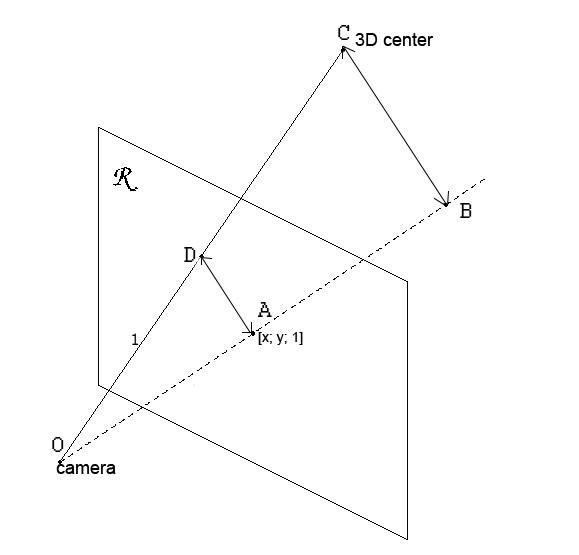
\includegraphics[scale=0.5]{3dcenter}
\caption{Вычисление трехмерных координат точек изображения}
\end{figure}

Таким образом, вычисляем трехмерные координаты всех углов отмеченных пользователем рамок. Далее можем вычислить трехмерную высоту и ширину выделенной рамки для каждого изображения. Считаем максимум среди этих расстояний. Полученное значение будем считать за сторону трехмерного куба, объемлющего объект.

\subsubsection{Инициализация вокселей, назначение каждому вокселю гипотез}
На следующем этапе для каждого изображения составляется матрица проекции:

\begin{center}
	$P = K*I*C$, где
\end{center}
$K$ - матрица внутренней калибровки камеры
$I$ - единичная матрица
$C$ - матрица внешней калибровки изображения.

Проекция воксела на изображение (координаты $x$ и $y$ в пикселях) получается умножением слева матрицы проекции данного изображения на трехмерный центр воксела:

\begin{center}
	$[x;y;z]^T = P*[X_{3D};Y_{3D};Z_{3D};1]^T$ \\
	$x = x/z$ \\
	$y = y/z$
\end{center}

Обходя все вокселы, для каждого воксела составляем гипотезы. Каждая гипотеза – это цвет проекции воксела на изображение в цветовом пространстве RGB. Для увеличения надежности алгоритма каждая компонента цвета гипотезы делится на сумму всех компонент (red + green + blue) этой гипотезы. Итого, для каждого воксела должно быть столько гипотез, сколько изображений во входной последовательности. Но если проекция воксела на изображение -- точка с пиксельными координатами $[x;y]$ -- выходит либо за границы изображения, либо за пределы выделенной пользователем рамки, соответствующая гипотеза считается ложной.

Сначала все вокселы видимые. Если все гипотезы для какого-либо воксела оказались ложными, этот воксел считается невидимым.

\subsubsection{Первоначальная отбраковка ложных гипотез}
Проходя последовательно по всем вокселам, для каждой гипотезы текущего воксела сравниваем ее со всеми остальными гипотезами для этого воксела. Гипотеза(1) считается верной, если найдется другая гипотеза(2) данного воксела, такая, что расстояние между этими гипотезами в цветовом пространстве RGB меньше заданного порога $T$:

\begin{center}
	$\lvert {red(0)} - {red(1)}\rvert + \lvert {green(0)} - {green(1)}\rvert + \lvert {blue(0)} - {blue(1)}\rvert < T$
\end{center}

Получим, что гипотеза ложная только в том случае, когда она не соответствует ни одной другой гипотезе для данного воксела. Так же как и ранее воксел считается невидимым, если все связанные с ним гипотезы ложны.

Далее считается, сколько осталось верных гипотез и изменяется порог $T$:

\begin{center}
	$T_{new} = T/{dim_x*dim_y*dim_z*N}$, где
\end{center}
$T_{new}$ - новое значение порога;\\
$dim_x, dim_y, dim_z$ - размерности результирующей модели по $x,y,z$ соответственно;\\
$N$ - количество изображений во входной последовательности.

Такое изменение порога позволяет более точно в дальнейшем определять ложные гипотезы.

\subsubsection{Дальнейшая проверка гипотез}

Алгоритм построен так, что он учитывает с какой стороны нужно рассматривать объемлющий куб для каждого изображения. Это сделано для того, чтобы правильно устанавливать видимость вокселей с каждого изображения. 

Чтобы найти порядок обхода вокселей для данного изображения, вычисляем расстояния в трехмерных координатах между камерой и всеми восемью углами объемлющего куба. Ближайший угол определяет порядок обхода вокселей: этот угол нужно обойти раньше остальных. 

В соответствующем порядке обходим куб и отбраковываем гипотезы как ранее:   
гипотеза ложная только в том случае, когда она не соответствует ни одной другой гипотезе для данного воксела, то есть:

\begin{center}
	$\lvert {red(i)} - {red(j)}\rvert + \lvert {green(i)} - {green(j)}\rvert + \lvert {blue(i)} - {blue(j)}\rvert > T_{new}$
\end{center}
при фиксированном $i$ для всех $i \neq j$.

Кроме того, для каждого изображения заводятся буфера – матрицы той же размерности, что и сами изображения на которых будут отмечаться видимые вокселы. Первоначально буфера пусты. Рассматривая каждую гипотезу проверяем, занят ли буфер на ее месте. Для этого вычисляем, какому вокселу соответствует эта гипотеза, Проецируем воксел на текущее изображение. Если буфер не занят, то заполняем его в тех  позициях, куда проецируется весь воксел (это может быть несколько пикселей). Если же буфер уже занят, то данный воксел не видим на этом изображении, и его гипотезу можно не рассматривать.    

Так обходятся все изображения в нужном порядке до тех пор, пока хоть одна гипотеза признается ложной. 

В итоге получаем вокселную модель реконструируемого объекта.

\newpage
\subsection{Реализация алгоритма}
Схематически алгоритм изображен на диаграмме ниже.
\begin{figure}[h]
\center
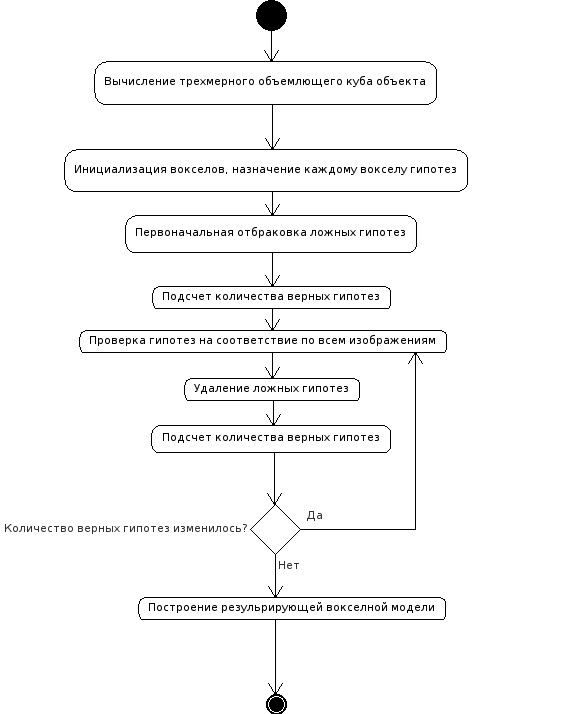
\includegraphics[scale=0.7]{qcovcactivitydiagram}
\caption{Диаграмма активности}
\end{figure}

На этапах <<Инициализация вокселей, назначение каждому вокселу гипотез>>, <<Первоначальная отбраковка ложных гипотез>>, <<Подсчет количества верных гипотез>> и <<Удаление ложных гипотез>> было применено распараллеливание вычислений.

\subsection{Приложение oclc}
Данное приложение является оберткой над компилятором OpenCL C. Оно позволяет проверить на корректность программы, написанные на языке OpenCL C и получить описание допущенных ошибок.

\subsection{Приложение qcovc}
Данное приложение позволяет пользователю, при помощи графического интерфейса, работать с библиотекой.

\subsubsection{Классы приложения}
\begin{itemize}
\item \textit{MainWindow} -- главное окно приложения
\item \textit{ImageInfo} -- информация об изображении
\item \textit{ImagePreview} -- виджет предпросмотра изображений
\item \textit{ImageScene} -- сцена для отображения изображения
\end{itemize}

\subsubsection{Класс MainWindow}
Методы класса:
\begin{itemize}
\item \textit{add\_image} -- добавление нового изображения
\item \textit{load\_metafile} -- загрузка метафайла
\item \textit{save\_metafile} -- сохранение метафайла
\end{itemize}

\subsubsection{Класс ImagePreview}
Методы класса:
\begin{itemize}
\item \textit{add\_image} -- добавление нового изображения в блок предпросмотра
\item \textit{clear} -- очистка блока предпросмотра
\end{itemize}

\subsubsection{Класс ImageScene}
Методы класса:
\begin{itemize}
\item \textit{rectangle\_changed} -- изменяет параметры объемлющего прямоугольника для изображения
\item \textit{set\_rectangle} -- устанавливает объемлющий прямоугольник для отображения
\item \textit{set\_image} -- устанавливает изображение для отображения
\end{itemize}

\subsubsection{Диаграмма классов}
\begin{figure}[h]
\center
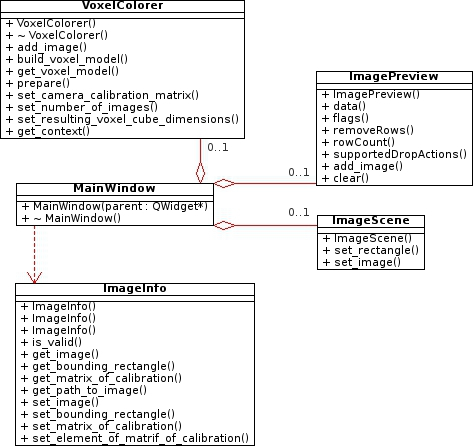
\includegraphics[scale=0.7]{qcovcclassdiagram}
\caption{Диаграмма классов приложения qcovc}
\end{figure}

\subsubsection{Проект интерфейса}
Из меню графического интерфейса пользователя должно быть доступно сохранение и загрузка метафайла, добавление нового изображения, запуск на выполнение алгоритма получения объемной модели объекта. Основное окно должно быть разделено на три части: слева должны находиться блок просмотра миниатюр изображений и блок ввода матрицы внешней калибровки камеры для выбранного изображения. Остальную часть окна должен занимать блок, в который выводится текущее выбранное изображение. Так же в этом блоке должно быть доступно выделение объемлющего прямоугольника.
\begin{figure}[h]
\center
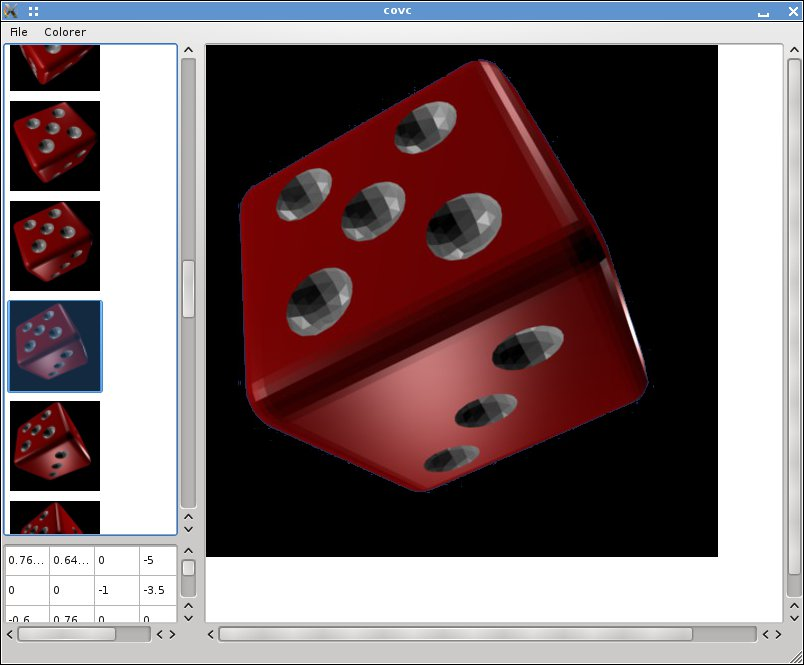
\includegraphics[scale=0.5]{gui}
\caption{Проект интерфейса}
\end{figure}

\newpage
\subsection{Приложение ocl\_volume\_render}
Данное приложение является модифицированной версией программы oclVolumeRender из комплекта NVIDIA GPU Computing SDK~\cite{nvidia_gpu_sdk} и позволяет пользователю просматривать полученную воксельную модель.



\section{Реализация и тестирование}
Объем итогового кода на С++ составляет 17.9 Кб в 12 файлах.\\
Объем автоматически сгенерированного кода (XML) составляет 3 Кб.\\
На текущий момент кодовая база содержит 4,693 строки.


\section*{Заключение}
В настоящий момент сделан набросок интерфейса, реализованы функции добавления изображения, загрузки метафайла, выделения основного объекта, ввода матрицы внешней калибровки камеры. В дальнейшем необходимо реализовать функцию сохранения метафайла, алгоритм построения воксельного объекта на основе изображений и введенных данных и функцию просмотра полученной воксельной модели объекта.



\renewcommand{\refname}{Список литературы}
\begin{thebibliography}{99}

	\bibitem{academic_free_license}
		Academic Free License ("AFL") v. 3.0 [Электронный~ресурс] : электрон.~энциклопедия -- Режим доступа:
		\url{http://www.opensource.org/licenses/academic.php}

	\bibitem{opencl_ati_support}
		ATI, ATI Stream Software Development Kit [Электронный~ресурс]
		 -- Режим доступа:
		\url{http://developer.amd.com/gpu/ATIStreamSDK/Pages/default.aspx#two}
	
	\bibitem{bsd}
		<<Simplified BSD License>> [Электронный~ресурс] : электрон.~энциклопедия -- Режим доступа:
		\url{http://www.opensource.org/licenses/bsd-license.php}
	
	\bibitem{chien}
		Chien C.H., Aggarwal J.K. Identification of 3D Objects from Multiple Silhouettes Using Quadtrees/Octrees // 
		Computer Vision Graphics And Image Processing -- 1986 -- PP. 256-273

	\bibitem{opencl_bindings}
		Experimental C++ Bindings to OpenCL [Электронный~ресурс] -- Режим доступа:
		\url{http://www.khronos.org/registry/cl/}
	
	\bibitem{foxc}
		Fixstars OpenCL Cross Compiler [Электронный~ресурс] -- Режим доступа:
		\url{http://www.fixstars.com/en/foxc/}
		
	\bibitem{opencl_ibm_support}
		IBM, OpenCL Development Kit for Linux on Power [Электронный~ресурс]
		-- Режим доступа:
		\url{http://www.alphaworks.ibm.com/tech/opencl}

	\bibitem{laser_scanner}
		Leica ScanStation 2 3D Laser Scanner [Электронный~ресурс] //
		FLT~Geosystems~website -- Режим доступа:
		\url{http://www.fltgeosystems.com/}

	\bibitem{multi_hypothesis}
		Eisert, P. Multi-Hypothesis, volumetric reconstruction of 3-d objects from multiple calibrated camera views /
		Peter Eisert, Eckehard Steinbach, Bernd Girod //
		ICASSP’99, Phoenix, USA -- march~1999. -- PP. 3509-3512

	\bibitem{opencl_standart}
		Khronos Group, OpenCL [Электронный~ресурс] -- Режим доступа:
		\url{http://www.khronos.org/opencl/}

	\bibitem{voxel_coloring_framework}
		Koen van de Sande, Voxel Coloring Framework [Электронный~ресурс]
		-- Режим~доступа:
		\url{http://voxelcoloring.sourceforge.net/}

	\bibitem{aggarwal}
		Martin W.N., Aggarwal J.K. Volumetric description of objects from multiple views //
		IEEE Transactions on Pattern Analysis and Machine Intelligence. -- 1983

	\bibitem{qt_qrectf}
		Nokia, QRectF [Электронный~ресурс]
		-- Режим доступа:
		\url{http://doc.trolltech.com/4.6/qrectf.html}

	\bibitem{qt_qstring}
		Nokia, QString [Электронный~ресурс]
		-- Режим доступа:
		\url{http://doc.trolltech.com/4.6/qstring.html}

	\bibitem{opencl_nvidia_support}
		NVIDIA, CUDA GPUs [Электронный~ресурс] -- Режим доступа:\\
		\url{http://www.nvidia.com/object/cuda_gpus.html}

	\bibitem{nvidia_gpu_sdk}
		NVIDIA GPU Computing SDK code samples [Электронный~ресурс] -- Режим доступа:\\
		\url{http://developer.nvidia.com/object/cuda_3_0GPU Computing SDK code samples_downloads.html}

	\bibitem{potmesil}
		Potmesil M. Generating Octree Models of 3D Objects from Their Silhouettes in a Sequence of Images // 
		Computer Vision Graphics And Image Processing -- 1987 -- PP. 1-29

	\bibitem{opencl_s3_support}
		S3 Graphics [Электронный~ресурс] -- Режим доступа:
		\url{http://www.s3graphics.com/}

	\bibitem{szeliski}
		Szeliski R. Rapid octree construction from image sequences // 
		Computer Vision, Graphics and Image Processing -- 1993 -- PP. 23–32
	
	\bibitem{bindings}
		Tkabber wiki, раздел <<Терминология>> [Электронный~ресурс] -- Режим доступа:
		\url{http://ru.tkabber.jabe.ru/}
	
	\bibitem{wiki_voxel}
		Воксел [Электронный~ресурс] : электрон.~энциклопедия -- Режим доступа: \url{http://ru.wikipedia.org/w/index.php?title=Voxel&oldid=22172795}

	\bibitem{wiki_crossplatfom}
		Кроссплатформенное программное обеспечение [Электронный~ресурс] : электрон.~энциклопедия -- Режим доступа:
		\url{http://wikipedia.org/}

	\bibitem{komarova_voxel_coloring}
		Комарова, Н. Практическая реализация алгоритма раскраски вокселей : курсовая работа / 
		Н.~Комарова~--~2005.~-~23 с.

	\bibitem{wiki_framework}
		Фреймворк [Электронный~ресурс] : электрон.~энциклопедия -- Режим доступа:
		\url{http://ru.wikipedia.org/wiki/Framework}

\end{thebibliography}



\end{document} % конец документа

